%        File: arfc-beamer.tex
%     Created: Sun May 5 10:00 PM 2013 C
%


%\documentclass[11pt,handout]{beamer}
\documentclass[9pt]{beamer}
\usetheme[white]{Illinois}
%\title[short title]{long title}
\title[Short Title]{A Very Very Long Title for a Presentation about Cats}
%\subtitle[short subtitle]{long subtitle}
\subtitle[Short SubTitle]{Mostly Kittens}
%\author[short name]{long name}
\author[Your Name]{Your Name\\Advanced Reactors and Fuel Cycles Group}
%\date[short date]{long date}
\date[04.01.2100]{April 1, 2100}
%\institution[short name]{long name}
\institute[UIUC]{University of Illinois at Urbana-Champaign}

%\usepackage{bbding}
\usepackage{amsfonts}
\usepackage{amsmath}
\usepackage{xspace}
\usepackage{graphicx}
\usepackage{subfigure}
\usepackage{booktabs} % nice rules for tables
\usepackage{microtype} % if using PDF
\usepackage{bigints}
\usepackage{tabularx}
%\usepackage{minted}

\newcommand{\units}[1] {\:\text{#1}}%
\newcommand{\SN}{S$_N$}%{S$_\text{N}$}%{$S_N$}%
\DeclareMathOperator{\erf}{erf}
%I need some complimentary error funcitons... 
\DeclareMathOperator{\erfc}{erfc}
%page numbers
\setbeamertemplate{footline}[page number]
\setbeamertemplate{caption}[numbered]
%Those icons in the references are terrible looking
\setbeamertemplate{bibliography item}[text]

%%%% Acronym support

\usepackage[acronym,toc]{glossaries}
\include{acros}

\makeglossaries

%try to get rid of header on title page\dots
\makeatletter
    \newenvironment{withoutheadline}{
        \setbeamertemplate{headline}[default]
        \def\beamer@entrycode{\vspace*{-\headheight}}
    }{}
\makeatother
\begin{document}
	%%%%%%%%%%%%%%%%%%%%%%%%%%%%%%%%%%%%%%%%%%%%%%%%%%%%%%%%%%%%%
	%% From uw-beamer Here's a handy bit of code to place at 
	%% the beginning of your presentation (after \begin{document}):
	\newcommand*{\alphabet}{ABCDEFGHIJKLMNOPQRSTUVWXYZabcdefghijklmnopqrstuvwxyz}
	\newlength{\highlightheight}
	\newlength{\highlightdepth}
	\newlength{\highlightmargin}
	\setlength{\highlightmargin}{2pt}
	\settoheight{\highlightheight}{\alphabet}
	\settodepth{\highlightdepth}{\alphabet}
	\addtolength{\highlightheight}{\highlightmargin}
	\addtolength{\highlightdepth}{\highlightmargin}
	\addtolength{\highlightheight}{\highlightdepth}
	\newcommand*{\Highlight}{\rlap{\textcolor{HighlightBackground}{\rule[-\highlightdepth]{\linewidth}{\highlightheight}}}}
	%%%%%%%%%%%%%%%%%%%%%%%%%%%%%%%%%%%%%%%%%%%%%%%%%%%%%%%%%%%%%
	%%--------------------------------%%
	\begin{frame}
	\frametitle{PyRe: Cyclus (Py)ro (Re)processing Module}
	\begin{columns}
		\begin{column}{.45\textwidth}
			\textbf{Current Work:} \\
			Create a class for each sub-process, and build the archetype. \\
			\vspace{1mm}
			\textbf{How does PyRe work?} \\
			PyRe does the following with an input stream and facility configuration parameters: 
			\begin{itemize}
				\item Fuel passed into voloxidation subprocess.
				\item A table of separation efficiencies is generated from input parameters.
				\item Input stream is multiplied by efficiency table to separate waste.
				\item Repeated for each process - results in product and waste composition streams.
			\end{itemize}
		\end{column}
		\begin{column}{.55\textwidth}
			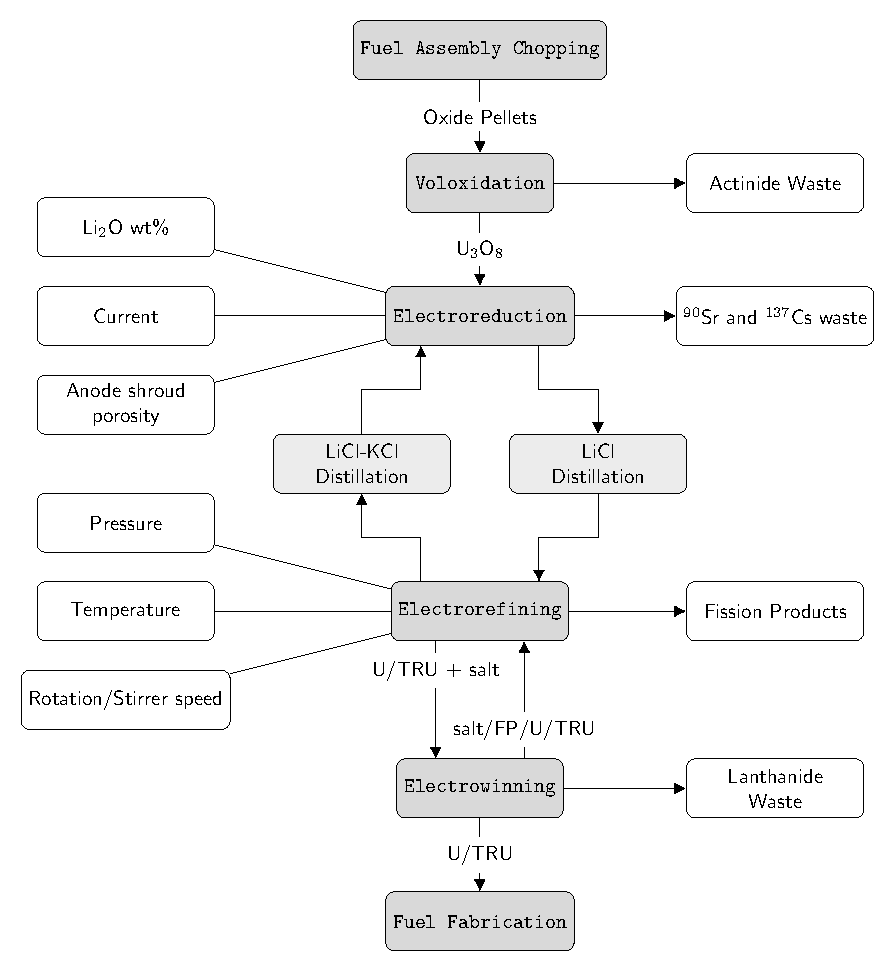
\includegraphics[width=\linewidth]{flowchart}
		\end{column}
	\end{columns}
	\end{frame}
	\begin{frame}
	\frametitle{PyRe: Cyclus (Py)ro (Re)processing Module}
	\textbf{Timeline:} \\
	The archetype will be functional with preliminary efficiencies early \textbf{August 2018}. \\
	A more detailed PyRe will be completed for ANTPC in \textbf{September 2018}. \\
	\vspace{1mm}
	\textbf{Archetype Uses:} \\
	PyRe will answer the following questions
	\begin{itemize}
			\item What is the affect of introducing pyroprocessing plants in the fuel cycle?
			\item How various facility designs affect throughput, efficiency and fabrication time?
			\item What are the best points to monitor a pyroprocessing plant for diversion?
	\end{itemize}
	\vspace{1mm}
	\textbf{Where is PyRe?} \\
	PyRe can be found in the "pyre" branch of recycle: \href{https://github.com/arfc/recycle}{arfc/recycle.} \\
	\vspace{1mm}
	\textbf{Who is working on this?}\\
	Greg Westphal, UIUC Graduate Researcher \\
	
	\end{frame}
\end{document}